% Chapter 2: Basic Concepts - From One-Hot to Dense Embeddings

\section{Basic Concepts}

% One-Hot Encoding
\begin{frame}{Starting Point: One-Hot Encoding}
\textbf{The Simplest Approach - But Fundamentally Flawed}

\begin{columns}
\column{0.5\textwidth}
\textbf{How One-Hot Works:}
\begin{center}
\begin{tabular}{|l|c|}
\hline
\textbf{Word} & \textbf{Vector} \\
\hline
cat & [1, 0, 0, 0, 0] \\
dog & [0, 1, 0, 0, 0] \\
mat & [0, 0, 1, 0, 0] \\
sat & [0, 0, 0, 1, 0] \\
hat & [0, 0, 0, 0, 1] \\
\hline
\end{tabular}
\end{center}

\textbf{Visual Representation:}
\begin{center}
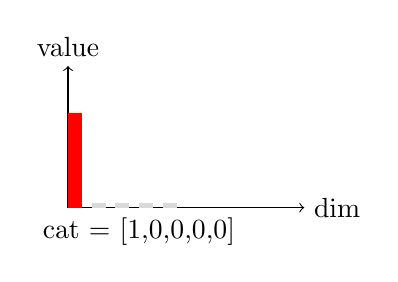
\begin{tikzpicture}[scale=0.6]
    % Draw axes
    \draw[->] (0,0) -- (5,0) node[right] {dim};
    \draw[->] (0,0) -- (0,3) node[above] {value};
    
    % Cat vector
    \fill[red] (0,0) rectangle (0.3,2);
    \fill[gray!30] (0.5,0) rectangle (0.8,0.1);
    \fill[gray!30] (1,0) rectangle (1.3,0.1);
    \fill[gray!30] (1.5,0) rectangle (1.8,0.1);
    \fill[gray!30] (2,0) rectangle (2.3,0.1);
    
    \node at (1.5,-0.5) {cat = [1,0,0,0,0]};
\end{tikzpicture}
\end{center}

\column{0.5\textwidth}
\textbf{Critical Problems:}

\begin{enumerate}
    \item \textbf{No Similarity:}
    $$\text{similarity}(\text{cat}, \text{kitten}) = 0$$
    $$\text{similarity}(\text{cat}, \text{computer}) = 0$$
    Both are equally dissimilar!
    
    \item \textbf{Huge Dimensions:}
    \begin{itemize}
        \item English: 170,000+ words
        \item Each word = 170,000-dim vector
        \item 99.999\% zeros (sparse!)
    \end{itemize}
    
    \item \textbf{No Relationships:}
    $$\text{cat} + \text{kitten} = [1,0,0...] + [0,1,0...] = [1,1,0...]$$
    Meaningless!
\end{enumerate}
\end{columns}

\vspace{0.2cm}
\begin{center}
\colorbox{yellow!20}{\parbox{0.8\textwidth}{
\textbf{Conclusion:} One-hot encoding treats all words as equally different - we need something better!
}}
\end{center}
\end{frame}

% Dense Embeddings Introduction
\begin{frame}{Dense Embeddings: The Solution}
\textbf{From Sparse to Dense - Capturing Meaning in Vectors}

\begin{columns}
\column{0.5\textwidth}
\textbf{The Transformation:}
\begin{center}
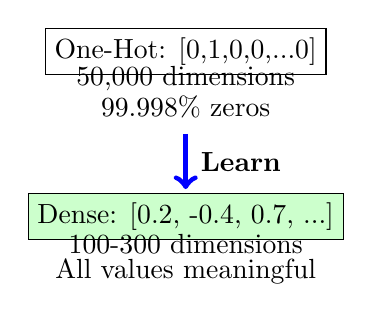
\begin{tikzpicture}[scale=0.7]
    % One-hot
    \node[draw, rectangle] (onehot) at (0,2) {One-Hot: [0,1,0,0,...0]};
    \node at (0,1.5) {50,000 dimensions};
    \node at (0,1) {99.998\% zeros};
    
    % Arrow
    \draw[->, line width=2pt, blue] (0,0.5) -- (0,-0.5);
    \node at (1,0) {\textbf{Learn}};
    
    % Dense
    \node[draw, rectangle, fill=green!20] (dense) at (0,-1) {Dense: [0.2, -0.4, 0.7, ...]};
    \node at (0,-1.5) {100-300 dimensions};
    \node at (0,-2) {All values meaningful};
\end{tikzpicture}
\end{center}

\textbf{Benefits:}
\begin{itemize}
    \item 100x smaller
    \item Captures semantics
    \item Enables arithmetic
    \item Learned from data
\end{itemize}

\column{0.5\textwidth}
\textbf{Visual Comparison:}
\begin{center}
\textbf{Sparse (One-Hot):}
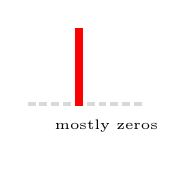
\begin{tikzpicture}[scale=0.5]
    \foreach \x in {0,0.3,...,3} {
        \fill[gray!30] (\x,0) rectangle (\x+0.2,0.1);
    }
    \fill[red] (1.2,0) rectangle (1.4,2);
    \node at (2,-0.5) {\tiny mostly zeros};
\end{tikzpicture}

\vspace{0.5cm}
\textbf{Dense:}
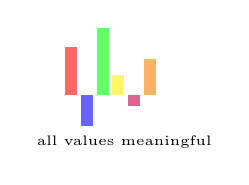
\begin{tikzpicture}[scale=0.5]
    \fill[red!60] (0,0) rectangle (0.3,1.2);
    \fill[blue!60] (0.4,0) rectangle (0.7,-0.8);
    \fill[green!60] (0.8,0) rectangle (1.1,1.7);
    \fill[yellow!60] (1.2,0) rectangle (1.5,0.5);
    \fill[purple!60] (1.6,0) rectangle (1.9,-0.3);
    \fill[orange!60] (2.0,0) rectangle (2.3,0.9);
    \node at (1.5,-1.2) {\tiny all values meaningful};
\end{tikzpicture}
\end{center}

\textbf{Example Vector:}
$$\text{cat} = [0.21, -0.43, 0.67, 0.15, -0.22, ...]$$
Each dimension captures some aspect of meaning
\end{columns}
\end{frame}

% Embedding Space Visualization
\begin{frame}{The Embedding Space: Where Words Live}
\textbf{Visualizing Word Relationships in Vector Space}

\begin{columns}
\column{0.6\textwidth}
\textbf{2D Projection of Word Vectors:}
\begin{center}
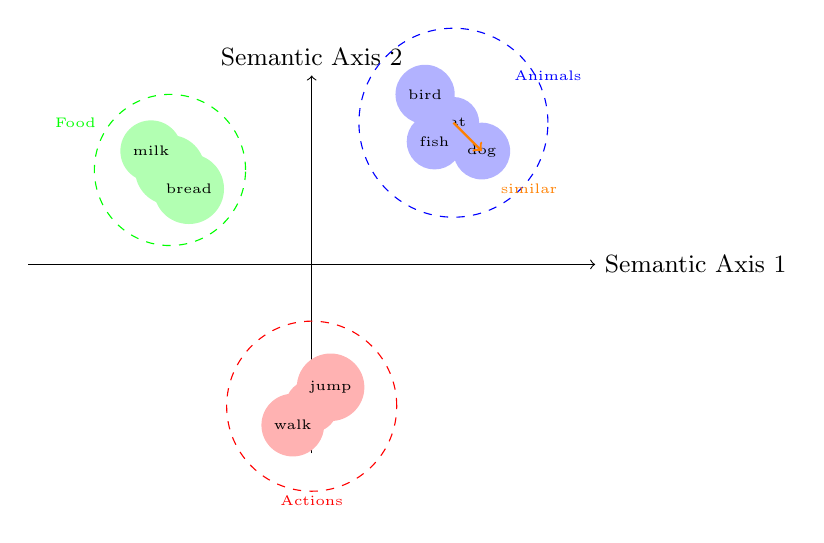
\begin{tikzpicture}[scale=1.2]
    % Draw axes
    \draw[->] (-3,0) -- (3,0) node[right] {\small Semantic Axis 1};
    \draw[->] (0,-2) -- (0,2) node[above] {\small Semantic Axis 2};
    
    % Animals cluster
    \draw[dashed, blue] (1.5,1.5) circle (1);
    \node[blue] at (2.5,2) {\tiny Animals};
    \node[circle, fill=blue!30] at (1.5,1.5) {\tiny cat};
    \node[circle, fill=blue!30] at (1.8,1.2) {\tiny dog};
    \node[circle, fill=blue!30] at (1.2,1.8) {\tiny bird};
    \node[circle, fill=blue!30] at (1.3,1.3) {\tiny fish};
    
    % Food cluster
    \draw[dashed, green] (-1.5,1) circle (0.8);
    \node[green] at (-2.5,1.5) {\tiny Food};
    \node[circle, fill=green!30] at (-1.5,1) {\tiny apple};
    \node[circle, fill=green!30] at (-1.3,0.8) {\tiny bread};
    \node[circle, fill=green!30] at (-1.7,1.2) {\tiny milk};
    
    % Actions cluster
    \draw[dashed, red] (0,-1.5) circle (0.9);
    \node[red] at (0,-2.5) {\tiny Actions};
    \node[circle, fill=red!30] at (0,-1.5) {\tiny run};
    \node[circle, fill=red!30] at (0.2,-1.3) {\tiny jump};
    \node[circle, fill=red!30] at (-0.2,-1.7) {\tiny walk};
    
    % Show a relationship
    \draw[->, thick, orange] (1.5,1.5) -- (1.8,1.2);
    \node[orange] at (2.3,0.8) {\tiny similar};
\end{tikzpicture}
\end{center}

\column{0.4\textwidth}
\textbf{Key Properties:}

\begin{enumerate}
    \item \textbf{Clustering:}
    Similar words group together
    
    \item \textbf{Distance = Similarity:}
    \begin{itemize}
        \item cat $\leftrightarrow$ dog: close
        \item cat $\leftrightarrow$ run: far
    \end{itemize}
    
    \item \textbf{Directions = Relations:}
    \begin{center}
    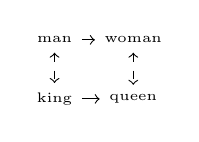
\begin{tikzpicture}[scale=0.5]
        \node (man) at (0,0) {\tiny man};
        \node (woman) at (2,0) {\tiny woman};
        \node (king) at (0,-1.5) {\tiny king};
        \node (queen) at (2,-1.5) {\tiny queen};
        
        \draw[->] (man) -- (woman);
        \draw[->] (king) -- (queen);
        \draw[<->, dashed] (man) -- (king);
        \draw[<->, dashed] (woman) -- (queen);
    \end{tikzpicture}
    \end{center}
    Gender direction is consistent!
\end{enumerate}
\end{columns}

\vspace{0.2cm}
\begin{center}
\colorbox{blue!10}{\parbox{0.9\textwidth}{
\textbf{The Magic:} The embedding space organizes itself to reflect real-world relationships!
}}
\end{center}
\end{frame}